%!TEX program = xelatex
% 完整编译方法 1 pdflatex -> bibtex -> pdflatex -> pdflatex
% 完整编译方法 2: xelatex -> bibtex -> xelatex -> xelatex
\documentclass[lang=cn,11pt]{elegantpaper}

\title{互联网金融风险与投资者风险意识 \\ {\large —— 来自网贷平台交易数据的证据}
\footnote{本文为~\href{https://github.com/ElegantLaTeX/ElegantPaper}{ElegantPaper} 的示例文档,最新版\href{https://github.com/EthanDeng/risk-awareness}{下载}。文章正式发表于《财贸经济》2019 年 第 2 期,本文仅供模板写作参考。}}
\author{\href{https://ddswhu.me/}{邓东升} \quad \href{http://www.cces.fudan.edu.cn/researchdetail.aspx?id=6}{陈钊}}

\institute{复旦大学 \; 经济学院 \\ 中国社会主义市场经济研究中心}
\date{2019 年 2 月 2 日}

\newcommand{\ekeywords}[1]{\vskip2ex\par\noindent\normalfont{\bfseries Key Words: }#1}

\begin{document}

\maketitle

\begin{abstract}
本文首次利用 575 家 P2P 网贷平台的运营数据,检验了投资者对网贷产品是否具备较强的风险意识。我们发现,无论是对于特定平台的个体风险,还是行业的整体市场风险,投资者的行为都表现出一定的风险意识:一方面,提高利率,缩短期限的确能吸纳更多的投资,但是对于潜在的问题平台,吸纳投资的效果明显更差,平台过高的利率甚至会使投资者减少投资;另一方面,当市场上有更多的网贷平台成为问题平台时,投资者的投资行为也会表现得更为谨慎。
\keywords{P2P 网络借贷 \; 问题平台 \; 市场风险 \;  风险意识}
\end{abstract}

\section{引言}

互联网金融是指传统金融机构与互联网企业依托互联网技术和工具,提供资金融通、支付、投资和信息中介服务的一种新型商业模式。根据 360 大数据平台,互联网支付和 P2P 网络借贷(简称 P2P 网贷)是互联网金融最受关注的两种业态。而 P2P 网贷的监管才刚起步,这为我们提供了一个较为难得的研究机会,能够考察在监管缺失的背景下互联网金融可能存在的风险以及投资者对这种新兴的金融业态具备怎样的风险意识。
P2P 网贷平台涉及三个行为主体,投资者、网贷平台、借款人,以及两项产品,投资理财产品和贷款。网贷平台具体的运营流程大致如下:在网贷平台上注册帐号的借款人可以向平台提出借款需求,并提供包括金额、用途、期限、利率等信息,以及相关的材料与证件,网贷平台对借款人提供的材料进行审核。一旦借款人被审核通过,平台将在其网站上发布散标或者打包成理财产品,散标或者理财产品满标后平台以贷款的形式向借款人放款。

P2P 网贷手续便利,一切认证、记账、清算和交割流程均通过网络完成,并且其贷款门槛远低于传统银行,因此这一新兴的金融模式自引入中国以来便迅速发展。自 2007 年 8 月首家 P2P 网络借贷平台——拍拍贷在上海成立以来,截至 2013 年底,运营平台数便达到了 800 家。图~\ref{fig:dev} 给出了 P2P 运营平台数量的发展变化。

\begin{figure}[htbp]
\centering
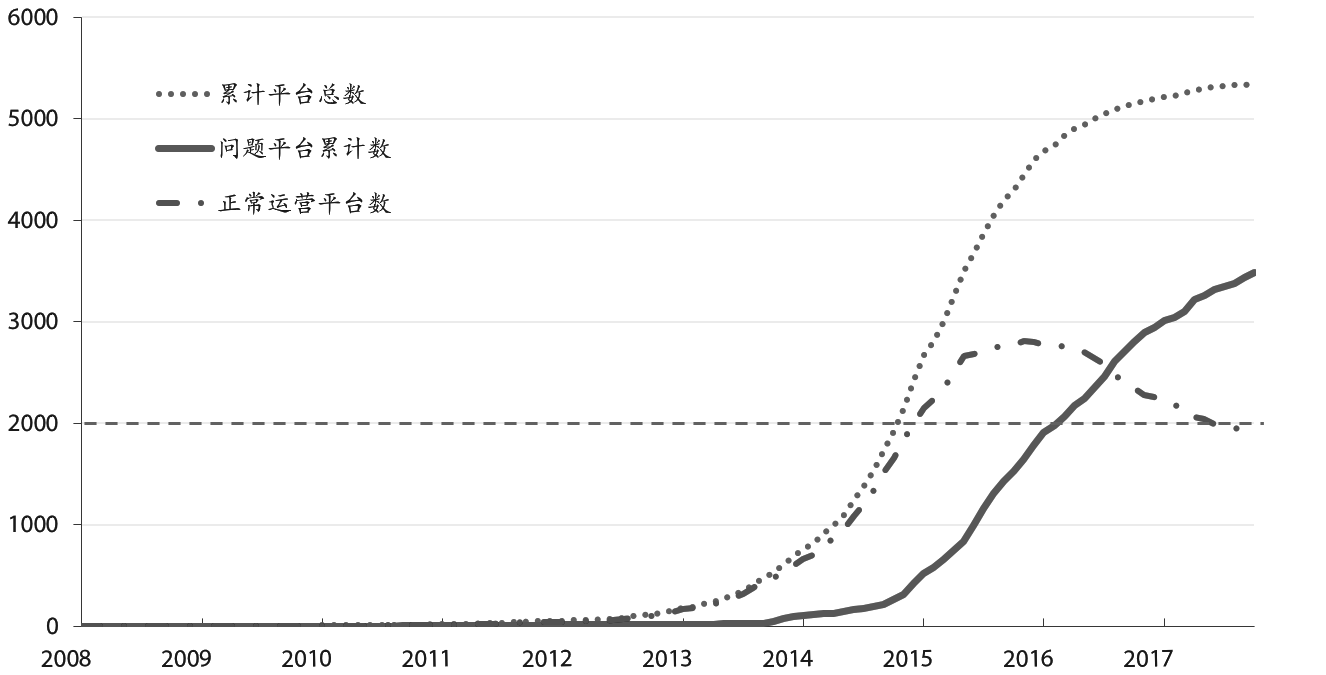
\includegraphics[width=0.7\textwidth]{figure/development_gray.png}
\caption{P2P 各月份累计平台数,问题平台数与正常运营平台数 \label{fig:dev}}
{\fontsize{8pt}{10pt}\selectfont\parbox{0.7\textwidth}{资料来源:零一数据}}
\end{figure}

但是,对于这一缺乏监管的新兴行业,担忧与质疑也同样存在。在众多网贷平台相继发生问题之后,2015 年 12 月 28 日,政府发布《网络借贷信息中介机构业务活动管理暂行办法(征求意见稿)》,并于 2016 年 8 月正式发布该办法,由此拉开了 P2P 网贷行业监管的序幕。从图 1 可见,受政府监管的影响,2016 年网贷平台数量的确在下降,并且平台数在 2017 年第四季度首次跌破 2000 家。不过,根据网贷之家的数据,P2P 网贷总的成交规模在稳步增长,仅在 2017 年第四季度略有下降。

各方面对 P2P 网贷的担忧可以归纳为以下三点。第一,网贷平台的利率较高,而央行一再表示,年复合利率超过银行利率 4 倍便不受法律保护 \footnote{银行定期利率(1 年期)大约为 1.5\%--2.25\%,而 P2P 行业综合年利率 2012 年为 23.43\%,2013 年为 24.93\%,2014 年为 17.52\%,2015 年为 12.05\%(银行利率数据:融 360《2017 年初 42 家银行的最新存款利率》;P2P 利率数据来源:第一网贷《2015 年全国 P2P 网贷行业快报》)。}。 第二,P2P 平台拥有资金帐户的调配权,而监管的缺乏可能导致平台出现挪用资金、卷款跑路的风险。第三,投资者对互联网金融这一新兴事物盲目追捧,缺乏必要的风险意识。网贷之家数据显示,从 2014 年起,问题平台数迅速增加,当年达到 275 家。 2016 年, P2P 行业内大规模的整改,问题平台数量进一步增加到了 1741 家 \footnote{问题平台的相关数据来源于:\href{http://www.wdzj.com/}{网贷之家}。}。

但是,到目前为止,学界对 P2P 网贷市场上投资者对于风险的认知与识别的研究仍较为初步。现有 P2P 研究内容主要涉及:
\begin{enumerate*}[label=(\arabic*)]
	\item 借款人或标的特征对于借贷结果的影响。其中借款人的特征包括外貌,年龄,人种~\citep{Ravina2008},信赖度~\citep{Duarte2012},还涉及到是否存在性别歧视或者地理歧视~\citep{lllmrwzw2014b,Komarova2015},标的的特征包括个人对标的的描述、借款用途描述、信用认证~\citep{lygyjlznczhwytyyx2014,phfzhyzy2016,ydzcx2017};
	\item 投资者投资决策的影响因素。主要考察了信任与风险感知对出借意愿的影响~\cite{cdyzhzhc2014},借贷风险的识别~\citep{lllmrwzw2014a},投资人所表现出的 “羊群效应”~\citep{lllmrwzwhpf2015},以及平台的保障体系对投资者投资决策的影响~\citep{lsxlh2015};
	\item P2P 平台投资收益率的决定因素以及利率特征,主要考察利率的形成机制,涉及到标的特征、宏观利率、借款人信用、借贷成本~\citep{Dietrich2016,cxydz2016},以及平台运营模式~\citep{chmyj2016} 对成交利率的影响,也考察了网贷市场利率的波动是否存在 “逆周期性”(陈霄和叶德珠,2016)。
	\item P2P 平台的风险与监管对策。目前大部分研究都集中于哪些特征(不随时间改变)的平台更容易成为问题平台~\citep{hypsywjy2016,wlfcxmm2014,wxhmloyh2016},也有部分围绕监管对策的定性分析~\citep{ajd2012,wj2015,Slattery2013}。
\end{enumerate*}
但上述研究都没有对网贷平台上投资者的风险意识提供直接的检验。与本文最为相关的研究是~\cite{lllmrwzw2014a} 对借贷风险的识别,他们发现,网贷产品的利率水平的确能够反映出产品未来违约风险的高低。与这项研究相比,本文对投资者风险意识的检验在以下两方面构成差异。第一,本文会根据网贷产品的特征直接度量平台的运营风险。第二,我们同时考察了投资者对平台的个体风险以及网贷市场整体风险的认知。

本文将以 575 家 P2P 网贷平台的微观运营数据为基础,考察投资者的投资行为是否显示出对所投资的网贷平台的运营风险以及网贷行业整体的市场风险有所认识。据我们所知,用这样的微观数据同时区分网贷平台的个体风险与网贷行业的整体风险,并考察投资者风险意识的实证研究在国内尚属首次。本文的主要发现是:
\begin{enumerate*}[label=(\arabic*)]
\item 高利率、短期限的平台,其运营风险也会越大;
\item 投资者对所投资的网贷平台的风险有所认识。具体而言,投资者在受平台产品高利率吸引而投资时,会对风险较高的潜在问题平台表现得更为谨慎。特别地,如果平台运营中体现出较高的风险(如该平台产品利率远高于网贷行业平均水平),则投资者会减少投资;
\item 投资者对网贷平台整体的市场风险也有认识。当市场上出现更多的问题平台时,投资者的投资行为也会更为谨慎。
\end{enumerate*}
本文的研究为我们判断投资者能否在监管缺失的环境下具备一定的风险意识提供了难得实证依据。
接下来本文第二部分介绍本文所使用的数据,第三部分是实证检验,最后是全文结论。

\section{数据与描述统计}

本文所使用的数据包括 3 个数据集,第一个数据集是平台的运营数据,主要来自网贷之家 \footnote{网贷之家是中国 P2P 业内最大、最权威、最具影响力的行业门户,汇集了较多 P2P 平台的运营数据。据我们所知,此网站数据是国内 P2P 平台运营数据唯一可得的来源,且覆盖面最广。} 网站上 575 家 P2P 网贷平台在 2014 年第 47 周到 2016 年第 32 周的非平衡面板数据,分为天数据、周数据两个数据集,其中大部分平台数据期限为 2015 年 32 周至 2016 年第 32 周。由于天的数据波动性较大,正文部分主要对周数据进行分析 \footnote{天数据的实证结果基本一致,如果需要可以向作者索要。} 。第二个数据集为平台层面的信息(6142 家平台,截止到 2018 年 4 月 1 日),主要来源于网贷之家,并利用网贷天眼上的信息进行校对。第三个数据集为平台的背景信息,主要来源于网贷天眼。数据获取主要是 Python 爬取和人工查询。

我们将本文所用数据与网贷行业的数据对比(2016 年 1 月 -- 2016 年 6 月)之后发现,虽然样本中正常运营平台数约为 500 家,仅占全行业数量的 1/6 不到,但样本中这些平台通常规模较大,运营稳定,因而总体市场份额较高。大致来看,本文样本中平台成交量占全行业 65\% -- 70\% 左右,资金净流入占全行业的 50\% -- 90\%。样本平台产品的平均期限比全行业大约多 1 -- 2 个月,平均利率大约低 1\% -- 2\%,这是由于风险较高规模较小的网贷平台通常不在我们的样本之中。虽然这也意味着,本文的结论并不宜做过多的外延推断,但如果我们能够发现投资者对这类相对较为安全的网贷平台仍然表现出风险意识,那么这个发现无疑是有意义的。此外,鉴于数据样本可得性,我们认为本文样本是目前可得的数据中,最能代表大部分正常运营平台的。

表~\ref{tab:var} 给出了上述数据库的主要变量及其解释,数据以周为单位。由于一周内投资者所购买的产品可能具有不同的限期与利率,因此表中的 “平均期限” 是指一周内所有投资产品的期限按各自本金金额的加权平均值,而 “平均利率” 则是一周内所有投资产品的利率按本金的加权平均值。 “资金净流入”这个变量也由平台直接提供,其取值相当于一周内的投资总额扣除平台偿还给投资人的金额(按本金计)。因此,用投资总额减去资金净流入,我们就可以得到平台一周内实际偿还给投资者的本金,我们称这一变量为 “实还本金”。以上变量均按照一周内的发生量来计算,我们将其列入表~\ref{tab:var} 的上半部分,而下半部分的变量则都是存量的概念。例如,“待还本金” 则是按特定时点上的存量信息来计算。我们根据平台是否出现资金流断裂、跑路(网站关闭,高层跑路)、停业、经侦介入等情形而区分问题平台与正常平台\footnote{当然,这里的正常平台也只是在我们的样本期内暂未出现问题的平台,因此下文我们在比较正常平台与问题平台的表现差异时,所得到的系数应该是一个下界。}。这个标准在国内两个最大的网贷门户网站——网贷之家与网贷天眼都是统一的,只是两个网站收录的网贷平台稍微有些差异,本文以网贷之家为准。为了度量网贷市场整体的投资风险,我们还计算了 “市场风险” 这个指标,即特定时间点前所有问题平台数除以总平台数(正常运营平台数 $+$ 问题平台数)。这个指标能反映出投资人能够感受到的网贷市场的整体风险。

% Table generated by Excel2LaTeX from sheet 'Sheet1'
\begin{table}[htbp]
\centering
\caption{核心变量与含义\label{tab:var}}
\begin{tabular}{llp{10cm}}
\toprule
变量    & 变量名   & 变量说明 \\
\midrule
投资人数  & $investors$ & 一周内投资该平台的人数(单位:人) \\
人均投资  & $investment\_pc$ & 一周内人均投资额(单位:万元) \\
投资总额* & $investment$ & 由 “投资人数” 与“人均投资”相乘得到(单位:万元) \\
平均利率  & $interest$ & 一周内平台投资产品利率的加权平均(单位:\%) \\
平均期限  & $term$  & 一周内平台投资产品期限的加权平均(单位:月) \\
资金净流入 & $net\_flow$ & 投资总额 – 本周内偿还投资者的金额(按本金计,单位:万元) \\
实还本金* & $repayment$ & 投资总额 – 本周平台资金净流入(按本金计,单位:万元) \\
\midrule
待还本金  & $to\_pay$ & 特定时点前所有借款人尚未偿还的本金总额(单位:万元) \\
问题平台 & $D_i$ & 平台出现无法提现、跑路、停业、经侦介入等,均被定义为问题平台,
否则视为正常平台(0~1 变量,其中 1 表示问题平台) \\
问题平台发生率* & $mkt\_risk$ & 特定时点前累计出现的问题平台总数 / 总平台数 \\
\bottomrule
\multicolumn{3}{p{12cm}}{\scriptsize 注:标 * 号的变量由平台提供的其它原始数据计算而得到。}
\end{tabular}%
\end{table}%


在 27285 个原始数据的基础上,删除待收投资人数与待还借款人数为负的样本(2 个),一周无任何投资额的样本(5 个),利率小于 1 的样本(13 个),剩余 27266 个有效样本。表~\ref{tab:sum} 给出了 575 个平台共计 27266 个样本观测值(平台 * 周)的所有变量描述统计。

% Table generated by Excel2LaTeX from sheet 'Sheet2'
\begin{table}[htbp]
\centering
\caption{主要变量的描述统计\label{tab:sum}}
\begin{tabular}{lrrrr}
\toprule
变量名   & 均值    & 标准差   & 最小值   & 最大值 \\
\midrule
投资人数  & 2125.66 & 8006.62 & 0     & 125307 \\
人均投资  & 6.02  & 58.31 & 0.01  & 5000 \\
投资总额  & 4092.46 & 16523.94 & 0.02  & 641949.8 \\
平均利率  & 13.76 & 4.39  & 1     & 53 \\
平均期限  & 4.23  & 4.84  & 0.03  & 54.26 \\
资金净流入 & 1206.63 & 9675.92 & -241202.20 & 565811.3 \\
实还本金  & 2885.83 & 11578.73 & 0     & 405045.8 \\
问题平台  & 0.26  & 0.44  & 0     & 1 \\
市场风险  & 0.25  & 0.12  & 0.1   & 0.47 \\
\bottomrule
\end{tabular}%
\end{table}%
    

\section{假说与实证检验}

接下来,我们将利用来自网贷平台的周面板数据回答本文所关心的问题。本文想要考察的是网贷市场上的投资者对于个体平台风险的识别以及对于整体市场风险的识别。因此,我们首先对上述两类风险进行衡量,然后对投资者的风险意识进行检验。

\subsection{平台风险与市场风险的衡量}

衡量平台风险的最直接指标是,看一个平台事后是否成为问题平台。如果一个平台最终成为问题平台,那么在其正常运营期间,它就是一个潜在的问题平台,我们认为该平台有较大的风险。衡量平台风险的另一个角度是找到能够体现个体平台运营风险的指标,为此,我们需要考察问题平台的特征。

从形式上来看,平台只是作为中介咨询机构,自身并非债务人。但是,由于平台对借款人有资质审核义务,并且大多数平台发布的并非散标,而是经平台打包组合后的理财产品, 平台在对债权打包时会出现期限错配,这就导致一旦某个借款人违约,这个单一债权所造成的风险可能传导到其它理财产品上。因此,如果平台因现金流压力过大而出现旗下产品不能向投资者如期还本付息,那么,平台的声誉必定会受影响。在流程上,平台也需要调用保证金账户中的保证金为投资人先行垫付。由此,我们预期在资金紧张时,类似于商业银行发布新的理财产品,网贷平台可能会通过策略性地操作增加平台的融资,例如,平台可能会通过发布更有吸引力(较高利率、较短期限)的理财产品来吸纳更多的投资。如果一个平台频繁出现这类策略性行为,那么平台的利率相对来说会比较高,这就提高了平台未来的还款压力,而且更短的期限也会加剧产品的期限错配,进一步增加运营风险。

表~\ref{tab:normalproblemsum} 则围绕几个核心变量对正常平台与问题平台进行了比较。我们可以发现,问题平台占比较小,其投资产品通常具有更高的平均利率,更短的平均期限,以及较小的规模,而且这种差异是显著的。

% Table generated by Excel2LaTeX from sheet 'Sheet3'
\begin{table}[htbp]
\centering
\caption{正常平台与问题平台比较\label{tab:normalproblemsum}}
\begin{tabular}{lccccc}
\toprule
      & 平均利率  & 平均期限  & 实还本金  & 投资总额  & 平台数 \\
\midrule
正常平台  & 12.87 & 4.62  & 201335.6 & 329836.30 & 412 \\
      & -3.41 & -5.06 & -668882.40 & -1123316.00 &  \\
问题平台  & 16.49 & 3.20   & 35208.54 & 43352.37 & 163 \\
      & -5.14 & -2.25 & -71224.09 & -85431.05 &  \\
差异    & 3.61*** & -1.42*** & -166127.10*** & -286484.00*** & 249 \\
\bottomrule
\multicolumn{6}{p{10cm}}{\scriptsize 注:括号内为标准差,并且 *** $p<0.01$, ** $p<0.05$, * $p<0.1$。}
\end{tabular}%
\end{table}%

由于一个网贷平台出问题主要有两类原因。第一类,平台在成立初期就是有缺陷的,甚至平台成立的目的就是为了圈钱,它们会利用高利率吸引更多的投资者,筹集到足够资金之后则携款跑路。第二类,平台迫于市场竞争压力,为了吸引投资者或者应对提现压力,发布了高利率、短期限的产品,结果导致后期更大的偿付压力,甚至因此成为问题平台。以上两类风险都可能通过高利率、短期限而表现出来。利率影响到后期的偿还压力,所以利率会影响到平台是否出问题是非常自然的。此外,很多平台为了解决借款人差异化的借款需求与投资者标准化产品需求,平台会涉及到期限错配,而错配会影响到平台的现金流,所以期限本身也会影响平台出问题的概率,加上期限也会通过利率影响到平台是否出问题。为此,我们设定如下实证回归(Probit 模型)来进一步检验利率与期限是否能够作为平台风险的度量:
\begin{equation}\label{eq:probit}
\begin{split}
      D_i & = \alpha + \beta interest_i + \gamma term_i + \delta X_i + \varepsilon_i \\
      D_i & = \alpha + \beta high\_interest_i + \gamma short\_term_i + \delta X_i + \varepsilon_i
\end{split}   
\end{equation}
其中 $D_i$ 表示截止到 2018 年 4 月 1 日,平台 $i$ 是否成为问题平台(问题平台取值为 1,否则取值为 0)。利率($interest$)与期限($term$)为平台在数据观测期间的平均利率与平均期限的分类变量,其中,利率取值为 1 -- 5,数值越大,利率越高,期限取值为 1 -- 7,数值越大,期限越长。而高利率($high\_interest$)和短期限($short\_term$)是哑变量,定义如下:平台在数据观测期间某一周平均利率高于 16\%,则高利率定义为 1,否则为 0。期限类似,如果平台在数据观测期间某一周平均期限比 3 个月更短,则短期限定义为 1,否则为 0。这两个变量衡量的是,在整个运营过程中,平台有没有出现过高风险的产品特征(高利率,短期限)。$X_i$ 为平台其他特征变量,其中包括注册资本与实缴资本。均为分类变量,取值为 1 -- 6,数值越大表示注册/实缴资本越大。我们利用这个回归来考察在整个样本期内发布高利率、短期限投资产品的平台是否在未来更可能成为问题平台。

表~\ref{tab:probit} 给出了回归方程~\eqref{eq:probit} 式的回归结果,被解释变量为平台是否为问题平台(问题平台 $=1$,正常平台 $=0$)。

\begin{table}[htbp]
\footnotesize
\centering
\caption{高利率、短期限与问题平台 Probit 回归\label{tab:probit}}
\begin{tabular}{lcccccc}
\toprule
      & (1) & (2) & (3) & (4) & (5) & (6)\\
\midrule
注册资本 & -0.146** &       & -0.257*** &       & -0.136** &  \\
      & (0.0595) &       & (0.0553) &       & (0.0606) &  \\
实缴资本 &       & -0.00206 &       & -0.126*** &       & 0.0116 \\
      &       & (0.0450) &       & (0.0396) &       & (0.0465) \\
利率 & 0.193*** & 0.202*** &       &       & 0.168*** & 0.174*** \\
      & (0.0546) & (0.0546) &       &       & (0.0571) & (0.0569) \\
期限 & -0.399*** & -0.428*** &       &       & -0.401*** & -0.435*** \\
      & (0.0549) & (0.0570) &       &       & (0.0572) & (0.0596) \\
高利率 &       &       & 0.462*** & 0.459*** & 0.247 & 0.294* \\
      &       &       & (0.142) & (0.142) & (0.162) & (0.163) \\
短期限 &       &       & 0.582** & 0.584** & 0.563* & 0.562* \\
      &       &       & (0.264) & (0.261) & (0.311) & (0.310) \\
常数项 & -0.202 & -0.786*** & -0.761** & -1.495*** & -0.843** & -1.436*** \\
      & (0.303) & (0.218) & (0.349) & (0.283) & (0.423) & (0.363) \\
样本 & 575 & 575 & 575 & 575 & 575 & 575 \\
\bottomrule
\multicolumn{6}{p{10cm}}{\scriptsize 注:括号内为标准差,并且 *** $p<0.01$, ** $p<0.05$, * $p<0.1$。}
\end{tabular}
\end{table}

在表~\ref{tab:probit} 中,我们是同时放入利率与期限两个因素进行回归的,但是我们试了把利率和期限依次放入回归方程,结果是一致的。从表~\ref{tab:probit} 可以看到,平台的注册资本/实缴资本越高,平台越可能是正常平台,这也很好理解,因为部分问题平台在成立初期就是打算短期集资,然后准备跑路,并不会提供更多的实缴资本。并且,资本实力越雄厚的平台,也更不可能因期限错配而出现运营问题。而我们核心关注的利率与期限这两个指标,的确能够用于度量平台未来的风险\footnote{度量平台风险的另一种做法是通过生存分析考察随时间变化的各种因素对风险的影响。由于下文中我们用于度量风险的指标(如~\eqref{eq:interest_diff} 式所示的利率差异指标)也是随时间变化的,为节省篇幅我们没有报告生存分析这部分内容,事实上结果是一致的。}。可以看到,利率越高,期限越短的平台更可能是问题平台,并且这个结果非常稳健。单看高利率和短期限的话,发行过非常高利率和非常短期限产品的平台更可能是问题平台。

但是,当我们直接用平台利率或期限度量特定平台的个体风险时,会受市场因素导致的利率或期限波动而干扰。因此,一个更合理的做法是用行业平均利率或行业平均期限对这种干扰加以剔除。平台利率与行业利率之间的差异以及平台期限与行业期限之间的差异可能是反映平台风险的两个重要因素\footnote{我们用生存面板分析进行了回归,由于过程相对繁琐,本文略过}。为了度量平台特征与行业整体水平的差异,我们计算了过去一段时间内平台利率(期限)与行业利率(期限)的差异,用该变量度量特定平台的个体风险。我们分别考虑了过去一周与过去一个月两种情形。本文的行业平均利率与平均期限都由月平均值来表示。对于利率差异($interest\_di\emph{f\kern0pt f}$)的计算公式如下(期限类似):

\begin{equation}\label{eq:interest_diff}
      interest\_di\emph{f\kern0pt f}_{it}(T) = \frac{1}{T} \sum_{\tau = 1}^{T} \big(interest_{i,t-\tau} - interest\_ind_{m(t-\tau)}\big)
\end{equation}

其中 $i$ 是平台,$t$ 为周,$m(t-\tau)$ 表示 $t-\tau$ 周所对应的月份,$interest$ 为平台的平均利率(周数据),$interest\_ind$ 为网贷行业的平均利率(月度数据)。$T$ 为滞后的阶数(周),本文 $T$ 的取值为 1 或者 4(作为稳健性检验)。当 $T=1$ 时,\eqref{eq:interest_diff}式计算的是过去一周,平台利率与行业利率之间的差异。当 $T=4$ 时,\eqref{eq:interest_diff}式计算的是过去一个月,平台利率与行业利率之间的差异。期限差异的计算方法与~\eqref{eq:interest_diff} 式类似,只是把利率指标换成期限。

为了度量网贷市场的整体风险,我们定义使用了问题平台发生率这个指标,指的是特定时间点前累计出现的问题平台数占全部平台数量的比例。使用这个指标能够较好地衡量网贷市场上投资者所能感知的市场整体风险,事实上,投资者可以通过网贷之家和网贷天眼获知问题平台发生率这个指标。

\subsection{投资者风险意识的检验}

在 P2P 网贷行业中,一个非常重要但至今仍缺乏相关证据的问题是:投资者是否具备风险意识?这又可以进一步分解为以下两个子问题:第一,投资者的投资行为是否能对所投资的特定平台的风险有所反应?第二,投资者的投资行为是否能对网贷市场的整体风险有所反应?如果投资者具备风险意识,那么针对第一个子问题我们提出以下待检验的假说:

\begin{enumerate}[leftmargin=7.2em]
\kaishu
\item[假说一: (a)] 潜在的问题平台更难以通过提高产品利率来吸纳更多投资。
\item[(b)] 当平台风险增加时,高利率或短期限产品吸纳投资的效果将减弱。 
\end{enumerate}

其中假说一 (a) 用是否潜在的问题平台度量平台个体风险,假说一 (b) 用利率与期限差异来度量平台的个体风险。

接下来,为了进一步检验投资者能否对网贷市场的行业风险有所识别,我们提出假说:

\begin{enumerate}[leftmargin=6em]
\kaishu
\item[假说二: ] 当网贷市场行业整体风险增加时,高利率或短期限产品吸纳投资的效果将减弱。
\end{enumerate}

为验证假说一 (a),我们对以下的回归模型按平台类型分别进行回归。
\begin{equation}\label{eq:interest}
      investment_{it} = \alpha + \beta interest_{it} + \gamma term_{it} + \delta X_{it} + \mu_i + \nu_t + \varepsilon_{it}
\end{equation}

其中,$i$ 为平台,$t$ 为时间(周),$investment$ 为投资总额,$interest$ 为平均利率,$term$ 为平均期限,$\mu_i$ 为平台固定效应,$\nu_t$ 为周固定效应。回归结果如表~\ref{tab:interest} 所示。

% Table generated by Excel2LaTeX from sheet 'Sheet3'
\begin{table}[htbp]
\centering
\caption{平台利率(期限)与平台融资\label{tab:interest}}
\begin{tabular}{lcccccc}
\toprule
      & (1)   & (2)   & (3)   & (4)   & (5)   & (6) \\
      & 全样本   & 正常平台  & 问题平台  & 全样本   & 正常平台  & 问题平台 \\
\midrule
平均利率  & 132.896*** & 200.134*** & 44.793*** & 0.008*** & 0.007*** & 0.005*** \\
      & (33.985) & (58.808) & (4.730) & (0.002) & (0.002) & (0.002) \\
平均期限  & -297.799*** & -367.461*** & -7.512 & 0.001 & -0.0001 & 0.009*** \\
      & (27.553) & (35.529) & (6.582) & (0.001) & (0.001) & (0.002) \\
常数项   & 2,010.981 & 2,582.378 & -182.762 & 2.721*** & 2.391*** & 2.464*** \\
      & (1955.597) & (7367.542) & (218.700) & (0.067) & (0.211) & (0.079) \\
样本数   & 27266 & 20239 & 7027  & 27266 & 20239 & 7027 \\
$R^2$    & 0.013 & 0.016 & 0.031 & 0.057 & 0.088 & 0.055 \\
平台数   & 575   & 412   & 163   & 575   & 412   & 163 \\
平台固定效应 & YES   & YES   & YES   & YES   & YES   & YES \\
周固定效应  & YES   & YES   & YES   & YES   & YES   & YES \\
\bottomrule
\multicolumn{7}{p{10cm}}{\scriptsize 注:被解释变量:投资总额或者 $\log_{10}(\text{投资总额})$(周)。}\\
\multicolumn{7}{p{10cm}}{\scriptsize 注:括号内为标准差,并且 *** $p<0.01$, ** $p<0.05$, * $p<0.1$。}
\end{tabular}%
\end{table}%
    

由于我们有很多不可观测的因素,平台自身特征可能会决定它所发布的产品的利率或者期限特征,我们需要通过时间固定效应,平台固定效应来尽可能的控制我们未观察到的因素以及不变的特征,来尽可能减少估计的误差。由列(1)可知,平均来看,提高利率或缩短期限的确能够使平台吸纳更多的投资。有意思的是,如列(2)、(3)所示,正常平台提高产品利率或缩短期限的融资效果远远大于问题平台。正常平台提高一个百分点的利率水平,能够多获得 200.1 万元投资总额,而问题平台仅能多吸纳 44.79 万元投资总额。这与我们的假说完全一致,说明投资者在问题平台问题暴露之前,就能够意识到该平台的潜在风险。对于问题平台,缩短期限对吸纳投资的效果并不显著,这既可能投资者风险意识的体现,也可能是因为,问题平台期限已经很短,想要进一步缩短期限来吸纳投资并不奏效。

由于不同类型平台的规模本身不一样,涉及的业务范围也相差很大(这会影响到产品利率和期限的结构),虽然我们控制了平台的固定效应,但是如果为了方便系数的比较,在(4)-(6)列中,我们换用投资额对数作为被解释变量。从(5)和(6)的对比可以看出,作为最直接的吸引投资的方法,提高利率确实能为正常平台吸纳更多的投资(百分比)。另外需要注意的是,对于问题平台,列(3)表明,缩短期限并不能吸纳投资,但是列(6)表明,如果问题平台缩短期限,吸纳投资的效果甚至是负的。这些证据都表明通过利率与期限,投资者其实对于潜在问题平台的风险是有识别能力的。

除了平台在样本期内是否成为问题平台这一信息之外,如前面的 Probit 回归所表明的那样,平台运营中的特征也可以用来衡量平台的风险。所以,接下来我们想检验假说一 (b),投资者能否识别平台自身风险的变化?

为了验证假说一 (b),我们将平台风险的度量 —— 平台与行业的利率差异($interest\_di\emph{f\kern0pt f}$)(期限差异类似)分别作为交互项加入到~\eqref{eq:interest} 式,得到:
\begin{equation}\label{eq:plat_risk}
      \begin{split}
            investment_{it} = \alpha &+ \beta interest_{it} + \beta' interest \times interest\_di\emph{f\kern0pt f}_{it}(T) \\
            &+ \gamma term_{it}  + \gamma' term \times term\_di\emph{f\kern0pt f}_{it}(T) + \mu_i + \nu_t + \varepsilon_{it}
      \end{split}
\end{equation}
其中,$i$ 为平台,$t$为时间(周),$\mu_i$ 为平台固定效应,$\nu_t$ 为周固定效应,平台与行业利率差异或者期限差异根据式~\eqref{eq:interest_diff} 计算。当平台与行业的利率差异增大,即平台的风险增加时,我们预期提高利率对吸引投资的效果将变差,即~\eqref{eq:plat_risk} 式中,利率前面的系数 $\beta$ 与交互项的系数 $\beta'$ 的符号应该相反,相应地,缩短期限对吸引投资的效果也会变差,即 $\gamma$ 与 $\gamma'$ 的符号也应该相反。类似地,当平台产品期限比行业产品的平均期限更短时,$term\_di\emph{f\kern0pt f}_{it}(T)$ 取值会更小,平台风险增加,提高利率或缩短期限对吸引投资的效果同样会减弱,因此我们预期将期限差异作为平台风险变量替换~\eqref{eq:plat_risk} 式中的利率差异时, $\beta$ 与交互项的系数 $\beta'$,以及 $\gamma$ 与 $\gamma'$ 的符号相同。

回归结果如表~\ref{tab:plat_risk} 所示。列(1)与列(2)使用过去一周平台利率(或期限)与行业利率(或期限)的差异来度量平台的运营风险。如列(1)所示,平台产品高利率、短期限对投资者资金的吸引会随着运营风险的上升(更高的利率差异)而下降。在列(2)中,运营风险由更小的期限差异来度量,结果仍然与我们的预期一致。如果我们用平台过去一个月的特征来度量平台的运营风险,如列(3)-(4)所示,回归结果仍然稳健。

% Table generated by Excel2LaTeX from sheet 'Sheet1'
\begin{table}[htbp]
\centering
\caption{平台风险与平台融资\label{tab:plat_risk}}
\begin{tabular}{lcccc}
\toprule
被解释变量 & (1)   & (2)   & (3)   & (4) \\
\midrule
投资总额(周) & \multicolumn{2}{c}{$T=1$} & \multicolumn{2}{c}{$T=4$} \\
\midrule
利率    & 46.043 & 204.419*** & 76.726 & 235.899*** \\
      & (51.160) & (36.954) & (51.076) & (37.011) \\
期限    & -306.645*** & -12.666 & -297.696*** & 18.171 \\
      & (28.639) & (35.371) & (28.172) & (34.051) \\
利率 $\times$ 利率差异 & -8.552*** &       & -10.959*** &  \\
      & (2.247) &       & (2.641) &  \\
期限 $\times$ 利率差异 & 99.101*** &       & 112.945*** &  \\
      & (6.550) &       & (6.869) &  \\
利率 $\times$ 期限差异 &       & 33.423*** &       & 42.336*** \\
      &       & (3.053) &       & (3.762) \\
期限 $\times$ 期限差异 &       & -47.433*** &       & -61.871*** \\
      &       & (1.953) &       & (2.194) \\
常数项   & 3726.802* & 2032.475 & 3446.041* & 1994.235 \\
      & (2058.117) & (1976.625) & (2036.982) & (1949.865) \\
样本数   & 26353 & 26353 & 26675 & 26675 \\
$R^2$    & 0.021 & 0.035 & 0.023 & 0.042 \\
平台数   & 575   & 575   & 575   & 575 \\
平台固定效应 & YES   & YES   & YES   & YES \\
周固定效应 & YES   & YES   & YES   & YES \\
\bottomrule
\multicolumn{5}{p{10cm}}{\scriptsize 注:括号内为标准差,并且 *** $p<0.01$, ** $p<0.05$, * $p<0.1$。}
\end{tabular}%
\end{table}%

为了检验假说二,即投资者对市场整体风险有所反应,我们设定如下回归方程:
\begin{equation}\label{eq:mkt_risk}
      \begin{split}
            investment_{it} = \alpha & + \beta interest_{it} + \beta ' interest \times mkt\_risk_{m(t)} \\
            & + \gamma term_{it} + \gamma ' term_{it} \times mkt\_risk_{m(t)} + \mu_i + \nu_t + \varepsilon_{it}
      \end{split}
\end{equation}
其中,$i$ 为平台,$t$ 为时间(周),$investment$ 为投资总额,$interest$ 为平台的平均利率,$term$ 为平台的平均期限,$mkt\_risk$ 为市场风险,$m(t)$ 表示 $t$ 周所对应的月份,$\mu_i$ 为平台固定效应,$\nu_t$ 为周固定效应,市场风险($mkt\_risk$)的度量是,$m(t)$ 月之前累计出现的问题平台数占全部平台数量的比例\footnote{我们也用了第 $t$ 期新增问题平台占正常运营平台数的比率作为市场风险的度量进行稳健性检验,我们还考虑了滞后一阶的效果,结论基本一致。}。我们预期交互项系数与对应一次项系数符号相反。回归结果如表~\ref{tab:mkt_risk} 所示。

% Table generated by Excel2LaTeX from sheet 'Sheet2'
\begin{table}[htbp]
\centering
\caption{市场风险与平台融资\label{tab:mkt_risk}}
\begin{tabular}{lcccc}
\toprule
      & (1)   & (2)   & (3)   & (4) \\
      & 所有平台  & 正常平台  & 问题平台  & 问题平台 \\
      &       &       &       & (限三个月前) \\
\midrule
平均利率  & 748.946*** & 1178.741*** & 63.311*** & 58.850*** \\
      & (94.365) & (152.751) & (15.292) & (18.848) \\
平均期限  & -1511.450*** & -1667.602*** & 36.327 & 67.886** \\
      & (81.007) & (100.004) & (28.514) & (34.191) \\
平均利率 $\times$ 市场风险 & -2103.143*** & -3177.454*** & -64.747 & -22.958 \\
      & (291.364) & (438.009) & (50.141) & (60.285) \\
平均期限 $\times$ 市场风险 & 3724.816*** & 3966.520*** & -137.922 & -293.827*** \\
      & (230.355) & (279.971) & (87.572) & (105.942) \\
常数项   & -2060.226 & -2480.977 & -465.656* & -889.043*** \\
      & (2191.305) & (7495.160) & (274.520) & (307.060) \\
样本数   & 27266 & 20239 & 7027  & 6229 \\
$R^2$    & 0.025 & 0.030 & 0.032 & 0.042 \\
平台数   & 575   & 412   & 163   & 161 \\
平台固定效应 & YES   & YES   & YES   & YES \\
周固定效应 & YES   & YES   & YES   & YES \\
\bottomrule
\multicolumn{5}{p{10cm}}{\scriptsize 注:括号内为标准差,并且 *** $p<0.01$, ** $p<0.05$, * $p<0.1$。}
\end{tabular}%
\end{table}%

表~\ref{tab:mkt_risk} 中列(1)的样本为全部平台,可以看到,系数显著为正的平均利率一次项表明更高的利率的确能够吸引更多投资。但是,平均利率与市场风险的交互项的系数也显著且符号与一次项刚好相反,这说明当网贷市场上整体的行业风险增加时,平台提高利率对投资者资金的吸纳效果就会显著变差。这就验证了假说二的成立,说明总体而言,投资者的投资行为会对市场的整体风险有所反应。产品平均期限这一变量的情况与此类似,也反映出市场风险提高后投资者对短期限产品变得更为谨慎。列(2)的回归只包含正常平台的样本,结果与全样本一致。

列(3)的回归只包含潜在问题平台,可以看到,问题平台的投资者与正常平台的投资者表现出较为明显的差异。此时,在我们关心的四个系数中,仅利率一次项显著为正,且该系数相对较小,这说明问题平台通过提高利率来吸引投资的效果较为有限,因而潜在问题平台的投资者对平台的风险有所认识。但是,列(3)中利率与市场风险的交互项并不显著,我们的猜想是,投资潜在问题平台的投资者很可能是一个比较特殊的群体,他们受平台的高利率吸引前来投资,但他们对该平台有着很强的风险认知,因此我们样本期中出现的市场整体风险的波动并不足以让他们的投资行为有明显改变。通过考察原始数据,我们发现,潜在问题平台在即将成为问题平台时其产品特征出现较大变化(如平均利率等变量的离散程度增加)。为此,我们进一步在列(4)的回归中,将潜在问题平台样本限制在出现问题的三个月以前。可以看到,利率及其交互项的回归结果与列(3)基本一致。在以上对假说二的检验中,如果我们用本周内新增问题平台数量占所有平台的比例来度量市场风险,结果仍然类似。

因此,通过对假说二的检验,我们的发现是,当网贷市场的行业整体风险增加时,投资者对高利率产品的投资会更加谨慎,并且,对市场风险的这一认识主要体现于正常平台的投资者。


\section{结论与启示}

本文利用来自 P2P 网贷平台的微观数据研究了在缺乏有效监管的环境下,投资者是否能够对潜在的风险有所识别。通过获取 575 家 P2P 网贷平台的运营数据,我们用是否为潜在的问题平台、平台产品利率或期限与行业产品利率或期限的差异来度量特定平台的个体风险,用市场上问题平台的比例来度量市场整体风险。我们发现投资者在受网贷产品更高利率吸引的同时,其投资行为对平台个体风险以及行业整体市场风险仍然表现出一定的风险意识。投资者对平台的风险意识表现为:
\begin{enumerate*}[label=(\arabic*)]
\item 潜在的问题平台更难通过高利率(短期限)吸引投资;
\item 当平台运营风险增加时,也就是平台利率(或期限)越来越高于(或短于)行业平均利率(或期限)时,投资者对高利率产品也会变得更为谨慎。
\item 当行业整体市场风险增加时,高利率(短期限)产品对投资者的吸引力也会显著减弱。    
\end{enumerate*}

本文的发现为我们认识 P2P 网贷市场投资者的风险意识提供了实证依据。由于 P2P 网贷是互联网金融的重要业态之一,本文的发现能够帮助我们理解快速发展的互联网金融所表现出来的投资风险以及在监管缺失的情况下,投资者对于互联网金融风险的把握。本文对于认识新兴金融业态的发展提供了政策依据。本文已经证实,即使在监管缺失的条件下,投资者仍然表对特定平台的个体风险与网贷行业的整体市场风险表现出明显的风险意识。这就意味着,政府虽然负有监管职责,但也不应轻易为投资者的损失“兜底”。此外,未来监管政策的基本思路应当是顺应市场的金融创新,在规范市场的同时,利用投资者的风险意识借助市场竞争实现网贷平台的优胜劣汰。

最后,本文的不足也是明显的。虽然本文的数据来源于网贷平台的交易数据,但回归中直接用的仍然是周或月的汇总信息,这有待未来有更细致的数据之后进一步改进。此外,对于潜在的问题平台,从我们的回归中可以看出,这类平台的投资者可能比较特殊,但受限于缺乏投资者的个人信息,我们无法进一步对潜在问题平台及其投资者作更深入的研究。最后,本文虽然证实了投资者在网贷平台的投资中表现出一定的风险意识,但我们无法判断这样的风险意识是否足够。

\bibliography{reference}

\begin{center}
{\Large \bfseries The Risk of Internet Finance and the Risk Awareness of Investors:\par}
{\large \bfseries Evidence from Transaction Data of P2P Online Lending Platforms \par}
{\large DENG Dongsheng, CHEN Zhao (Fudan University, 200433)}
\end{center}

\renewcommand{\abstractname}{Abstract}

\begin{abstract}
This paper examines the existence of risk awareness of investors in the 575 P2P platforms in China. We find that investors are aware of risk relating to particular platform as well as that from the market. On one hand, although investors prefer short-term and high-interest products, it is less effective for the potential problem platforms to attract investors. On the other hand, when more P2P platforms became problem ones, investors will be more cautious.
\ekeywords{P2P online Lending, Problematic Plat, Market Risk, Risk Awareness}
\end{abstract}


\end{document}
